\chapter{Neural network design}
\section{Architecture}
\begin{description}[style=unboxed]
    \item[How many input neurons are needed for this assignment?]
    There are 10 numerical values for features of the objects, so it's natural to use 10 input neurons.
    \item[How many output neurons do you require?]
    There are 7 possibilities of classes. We could define a value for every one of these classes and use 1 output neuron and train it to output the specific we want for every class. However a more logical choice would be having 7 output neurons, where we associate every output neuron with a specific class. In this way we can train the network to output a 1 on the related output neuron for an object of specific class and 0 on the other 6 neurons.
    \item[How many hidden neurons will your network have?]
    An amount of hidden neurons which is around the same as the amount of input and output neurons is generally accepted as a good practice. So we will start with using 8 hidden neurons.
    \item[Which activation function(s) will you use?]
    We will want our model to be non-linear, because we can't assume anything about the shape of the solution space. So the likely candidate is the logistic function. Another possibility is using tanh, which could be tested if the logistic function is found to not provide a good enough performance.
    \item[Give a schematic diagram of your complete network]
    \end{description}
    \tikzset{%
  every neuron/.style={
    circle,
    draw,
    minimum size=0.8cm
  },
  neuron dots/.style={
    draw=none, 
    scale=2,
    text height=0.333cm,
    execute at begin node=\color{black}$\vdots$
  },
}

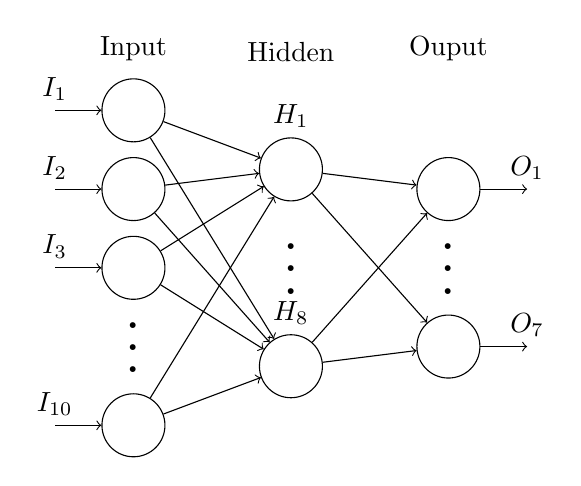
\begin{tikzpicture}
\foreach \m [count=\y] in {1,2,3,dots,4}
  \node [every neuron/.try, neuron \m/.try] (input-\m) at (0,2.5-\y) {};

\foreach \m [count=\y] in {1,dots,2}
  \node [every neuron/.try, neuron \m/.try ] (hidden-\m) at (2,2-\y*1.25) {};

\foreach \m [count=\y] in {1,dots,2}
  \node [every neuron/.try, neuron \m/.try ] (output-\m) at (4,1.5-\y) {};

\foreach \l [count=\i] in {1,2,3,10}
  \draw [<-] (input-\i) -- ++(-1,0)
    node [above] {$I_{\l}$};

\foreach \l [count=\i] in {1,8}
  \node [above] at (hidden-\i.north) {$H_{\l}$};

\foreach \l [count=\i] in {1,7}
  \draw [->] (output-\i) -- ++(1,0)
    node [above] {$O_{\l}$};

\foreach \i in {1,2,3,4}
  \foreach \j in {1,2}
    \draw [->] (input-\i) -- (hidden-\j);

\foreach \i in {1,2}
  \foreach \j in {1,2}
    \draw [->] (hidden-\i) -- (output-\j);

\foreach \l [count=\x from 0] in {Input, Hidden, Ouput}
  \node [align=center, above] at (\x*2,2) {\l};

\end{tikzpicture}

\section{Training}
\begin{description}[style=unboxed]
    \item[How and why did you divide your data into a training, validation and test set?]
    The division into a training, validation and test set is needed because if you just use a training set you'll have no reasonable way to know when to stop training, because using it itself as the validation set will generally give a lower error, so could stop training too quickly. So we will need a validation set for determining the end of the training.\\
    To also gain a measure of the error in classifying new unknown objects we will need another set for which we already know the real class. However if we've already used this set as validation or training set this could again give a falsely high estimate of expected error. For the training set this is obvious, and the validation set will only stop training when the network is decently good at classifying it, so using that as the test set would also give a false impression of how good the network functions, because by definition it'll already have a low error.\\ 
    In choosing the sizes for validation and tests sets we will want to make sure that we still have a large enough training set, while the training and validation sets will need to be large enough that we can expect that a good performance on them will likely also signify a good performance on any general input. For this we chose to use 500 of the known objects as validation data and 500 as testing data.
    \item[How do you evaluate the performance of your network?]
    We examine the summed square errors for the network over the validation set. Another possibility is using the amount of cases in which the actual class of the object in the test set was the highest output in the network, because that's how we will decide our classification after the training. However the sum squared error gives a more general picture of the likelihood of correct classification and so we will use that.
    \item[When and why do you decide to end the training?]
    We will again use the summed squared error as a measure of merit. Now the network will eventually reach a point where further training does not really change the error anymore, we will use this in our determination by stopping training if the mean square error on the validation set has decreased less than 10 percent over 5 epochs, these values might require further tweaking pending more tests.
    \item[Train your network 10 times, each with different initial weights. How does the initialization impact the performance?]
    It doesn't have any significant effect on the minimum sum squared error that is reached, however it does have a small effect on the speed of convergence to this minimum, it could take 3 epochs less. It also had an effect on which objects it classified incorrectly, which immediately makes you think of using multiple networks started with different initialisations and then taking classification that is given most frequently for a given object as it's actual classification. Doing this with the test set showed in increase from on average 450/500 correct to 465/500.
\end{description}


\section{Optimization}
\begin{description}[style=unboxed]
    \item[Generate a plot of the final performance versus the number of hidden neurons in the network.]
    In figure \ref{NeuronError} a measure of the error for different number of hidden neurons is given. The differences in results are quite small, all we can seriously conclude is that having just 7 neurons leads to a slightly larger error. Still 25 neurons gave the smallest error, and we won´t have to use the network in real time so computational time doesn´t matter much, so we´ll use 25 hidden neurons.
    \begin{figure}[h!]
  \centering
    \includegraphics[width=0.6\textwidth]{images/ErrorNeuroncount.png}
    \caption{Graph of the mean square error at the end of training for various numbers of hidden neurons}
    \label{NeuronError}
\end{figure}
\item[Show a plot of the performance of the
training set and the validation set during training, across epochs.]
    In figure \ref{epochserror} the error over 80 epochs is shown for both the training and validation set. It can be seen that the mean square error on the validation set always remains higher than the training set, as we would expect, but it also seems to stop decreasing before the error for the training set stops decreasing.
    \begin{figure}[h!]
  \centering
    \includegraphics[width=0.6\textwidth]{images/errorOverEpochs25Hidden.png}
    \caption{Graph of the mean square error over 80 epochs}
    \label{epochserror}
\end{figure}
\end{description}

\section{Evaluation}
\begin{description}[style=unboxed]
    \item[What is the success rate of your network on the test set? How does it compare to the
results of the validation set?]
    On a test set with 1000 elements the network manages on average around 925 correct classifications, on the validation set a similar number is reached, there doesn't seem to be any significant difference. This is to be expected from the way the error on the validation set steadily goes down on subsequent epochs and never goes back up.\\
    If the error for the validation set sometimes went up and sometimes down it could provide significant biasing for the success rate on the validation set by stopping the training right at a point where the error for the validation set is low. But because it just very smoothly goes down and then stays the same we can't get "unlucky" by by chance having a higher error than normal on the test set at the moment we stop training, because the mean square error over epochs quickly goes down to a certain base line and then stays the same in training as we saw in figure \ref{epochserror}.
      \item[Show a confusion matrix of your test set.]
     In figure \ref{confusion} the confusion matrix can be seen for the test set fed into our neural network. In it we can see which classes the objects of certain classes are classified as by the neural network. It can for example be seen that nearly all the objects that actually belong to class 2 were correctly classified as belonging to class 2, and that there were also very few objects classified as being of class 2 that actually belonged to a different class, so putting those 2 things together we can say that classifying objects of class 2 is going quite well.\\
     Now we can also see that in 11.5\% of the cases objects of class 3 were actually classified as belonging to other classes, which is quite a poor score, while 8.2\% of the objects classified as class 3 actually weren't of class 3, so we can say that the neural network does a very poor job of in classifying objects of class 3. Only in 3 cases does there seem to be any significant bias in the classification errors, namely objects of class 4 were commonly classified as being of class 7 while objects of class 7 were also commonly classified as being of class 4, while the results aren't very conclusive due to the small absolute amount of errors we are examining here, this might point to a strong similarity in the inputs related to class 4 and 7. And objects of class 3 were often mistaken to be of class 5, but not the other way around. Except for those special cases the errors seem to just be randomly spread, and even the ones mentioned could just be coincidence due to the small sample sizes.
    \begin{figure}[h!]
  \centering
    \includegraphics[width=0.6\textwidth]{images/confusionmatrix.png}
    \caption{The confusion matrix for the test set}
    \label{confusion}
\end{figure}
\end{description}

\section{MATLAB's Toolbox}
\begin{description}
    \item[Comment on the differences between your network's performance and the Toolbox.]
    A plot of the toolbox's error during training can be seen in figure \ref{toolbox}. It can be noted that the error's turn out to be quite a bit lower in the end, however on examining the outputs of the network we found that the output with the highest value corresponded to the correct output in 933 out of 1000 cases, which isn't at all significantly different from 925 out of 1000 correct maximum outputs for our own network, so the error for the case it gets correct is smaller, but it still gets about as many cases incorrect. So basically the toolbox gives a more complete picture of how much is certain for the classification of certain objects than our network. The time taken in training was also quite similar, with the toolbox training slightly faster.
    \begin{figure}[h!]
  \centering
    \includegraphics[width=0.6\textwidth]{images/toolboxErrorPlot.png}
    \caption{Plot of mean square error for MATLAB's neural network toolbox training}
    \label{toolbox}
\end{figure}
\end{description}
    
    
    
    
    
    
    
    
    
    
    
    
    
    
    
    